\section{Множества и логика}
\label{sec:sets}

\defemph{Множество}~--- ещё один низкоуровневый объект математики, который трудно определить строго.
Формально, в наше время множеством называют объект, удовлетворяющий определённой системе аксиом\footnote{Аксиоматическая теория множеств, система аксиом ZF.}.
Однако в ходе этого курса так глубоко копать не придётся: нам будет достаточно лишь сравнительно неформального определения множества.

\subsection{Теория множеств}
\label{subsec:sets:theory}

\begin{definition}
    \defemph{Множеством} называют совокупность неповторяющихся объектов без указания отношения между ними.
\end{definition}

Для краткости утверждение <<элемент $ x $ принадлежит множеству $ A $>> обозначают как $ x \in A $.
Аксиоматически полагается существование \defemph{пустого множества} (то есть, множества, которому не принадлежит ни один элемент), которое обозначают $ \varnothing $.

Множества можно задавать различными способами:
\begin{enumerate}[label=\arabic*)]
    \item
        Перечислением всех элементов: $ A = \{1, 2, 4\} $.
    \item
        Перечисление посредством правила:
        \[
            \N_0 = \{ 0, 1, 2, \ldots \}, \qquad \Z = \{\ldots, -2, -1, 0, 1, 2, \ldots \} = \{0, 1, -1, 2, -2, \ldots \}
        \]
        \textit{Понятно, что данный способ неприменим, если из перечисления читателю угадать правило невозможно.}
    \item
        \label{itm:sets:condition}
        Задание условием:
        \[
            \{ x \mid f(x) \} = \text{<<множество всех $ x $, для которых верно высказывание $ f(x) $>>}
        \]
        Пример:
        \begin{equation}
            \label{eq:sets:example_formula}
            [0; 1) = \{ x \mid (x \geqslant 0) \wedge (x < 1) \}
        \end{equation}
        \[
            \Q = \left\{ \frac{m}{n} \, \middle | \, m \in Z, \; n \in \N \right\}
        \]
\end{enumerate}

Последний способ вызвает некоторые вопросы; в частности, какие $ x $ <<пойдут на вход>> условию $ f(x) $.
Верно ли, например, что $ \sqrt{2} \in \{ x \mid \text{<<$ x $ не делится на $ 2 $>>} \} $?
А то, что $ \text{``стул''} \in \{ x \mid \text{<<$ x $ не делится на $ 2 $>>} \} $?
Для того, чтобы обойти эти трудности, вводится понятие множества всех элементов, или полного множества, или \defemph{юнивёрсума}, которое обычно обозночают $ U $.

\begin{definition}
    \defemph{Юнивёрсум}~--- множество всех элементов, на которых происходит проверка условия при соответствующем задании некоторого множества.
\end{definition}

Очевидно, что изначально нет никаких ограничений в выборе юнивёрсума; этот выбор обусловлен лишь постановкой задачи.
Поэтому требуется оговаривать заранее, что такое множество $ U $, или хотя бы упоминать его при каждом задании множества условием:
\[
    \{ x \in U \mid f(x) \} \qquad (\text{например,} \; [0; 1) = \{ x \in \R \mid (x \geqslant 0) \wedge (x < 1) \} )
\]

Множество~--- настолько фундаментальный объект, что с его помощью даже пытались описать всю математику.
\begin{example}
    С помощью множеств можно определить, что такое упорядоченная пара:
    \[
        (x, y) = \left\{ x, \{y\} \right\}
    \]
    Или что такое натуральные числа:
    \[
        \varnothing, \; \{ \varnothing \}, \; \left\{ \varnothing, \{ \varnothing \} \right\}, \; \left\{ \varnothing, \left\{ \varnothing, \{ \varnothing \} \right\} \right\}, \ldots
    \]
\end{example}

Однако камнем, на который нашла коса теории множеств, оказался, по сути, всё тот же юнивёрсум.

\begin{example}[Парадокс Рассела]
    Назовём некоторое множество <<обычным>>, если оно не содержит себя в качестве элемента.
    Пусть $ U_0 $~--- множество всех <<обычных>> множеств.
    Можно проверить, что не выполнено как $ U_0 \in U_0 $, так и $ U_0 \notin U_0 $, что является парадоксом.

    Заметим, что запрет на существование <<необычных>> множеств сильно обедняет теорию, ведь тогда не будет сущестовать юнивёрсум всех множеств.
\end{example}

Данный парадокс можно решить, лишь отказавшись от теории множеств в пользу более фундаментальной теории~--- теории типов, но это уже совсем другая история.



\subsection{Множества и логика}
\label{subsec:sets:logic}

Исследуя базовые понятия теории множеств, мы совсем не рассматривали операции, которые можно над множествами совершать.
В этом разделе мы убьём сразу двух зайцев: исследуем связь алгебры логики и теории множеств, а также, наконец, определим упомянутые операции.

Вернёмся к определению множества посредством задания условия.
Понятно, что если юнивёрсум~--- $ \{ 0, 1 \} $, то $ f(x) $ в пункте \ref{itm:sets:condition}~--- булева функция.
В более общем случае говорят, что $ f(x) $~--- \defemph{унарный предикат}.

\begin{definition}
    \defemph{Предикатом} арности $ n $ называют булевозначную функцию от $ n $ аргументов из $ U $. %из $ U^n $ в $ \{ 0, 1 \} $, где
    %\[
    %    U^n = \underbrace{U \times U \times \ldots \times U}_{n \; \text{раз}} = \text{<<множество всех кортежей длины $ n $ из элементов $ U $>>}
    %\]
\end{definition}

Аналогично булевым функциям, сложные предикаты можно конструировать из простых при помощи формул и логических связок (см. \eqref{eq:sets:example_formula}).
Однако наличие юнивёрсума позволяет использовать при построении предикатов ещё более мощный инструмент~--- \defemph{кванторы}.
Ограничимся лишь неформальным их определением:
\begin{align*}
    \forall \; (\text{всеобщности}): &\quad \forall x \, P(x) = \text{<<для любого $ x \in U $ истеннен предикат $ P(x) $>>} \\
    \exists \; (\text{существования}): &\quad \exists x \, P(x) = \text{<<существует $ x \in U $ такой, что истеннен предикат $ P(x) $>>}
\end{align*}

\begin{remark}
    В случае, когда юнивёрсум конечный, любую формулу с кванторами можно заменить эквивалентной формулой без них, используя связки $ \wedge $, $ \vee $ и $ \neg $.
    В общем случае это не так.
\end{remark}

%Без доказательства также приведём следующее замечание:
\begin{remark}[Обобщённый закон де Моргана]
    Справедливо равенство
    \[
        \forall x \, P(x) = \neg \left( \exists x \, \neg P(x) \right)
    \]
\end{remark}

Наконец, можно установить соответствие между любым множеством и некоторым предикатом:
\begin{equation}
    \label{eq:sets:indicator}
    A = \{ x \mid f(x) \} \qquad \Longleftrightarrow \qquad f(x) = \text{<<$ x \in A $>>}
\end{equation}

Предикат, соответствующий согласно равенству \eqref{eq:sets:indicator} некоторому множеству $ A $, будем называть \defemph{индикаторной функцийей} $ A $ и обозначать $ \I_A(x) $.
Используя индикаторные функции и алгебру логики,
можно определить все привычные и непривычные вам теоретико-множественные операции (таблица \ref{tab:sets:operations}) и отношения (таблица \ref{tab:sets:relations}).
Заметим, что пустое множество является подмножеством любого множества!

\begin{table}[ht!]
    \center
    \begin{tabular}{|c|c|c|c|}
        \hline
        Название & Обозначение & Описание & Формула \\
        \hline
        \hline
        Пересечение & $ A \cap B $      & \makecell{Элементы, входящие \\ как в $ A $, так и в $ B $}      & $ \I_{A \cap B}(x) = \I_A(x) \wedge \I_B(x) $ \\
        Объединение & $ A \cup B $      & \makecell{Элементы, входящие \\ в $ A $ или $ B $}               & $ \I_{A \cup B}(x) = \I_A(x) \vee \I_B(x) $ \\
        Разность    & $ A \setminus B $ & \makecell{Элементы, входящие \\ в $ A $, но не в $ B $}          & $ \I_{A \setminus B}(x) = \I_A(x) \wedge \neg \I_B(x) $ \\
        \makecell{Симметрическая \\ разность} & $ A \symdiff B $ & \makecell{Элементы, входящие \\ либо в $ A $, либо в $ B $} & $ \I_{A \symdiff B}(x) = \I_A(x) \oplus \I_B(x) $ \\
        Дополнение  & $ A^c, \; U \setminus A $ & \makecell{Элементы юнивёрсума, \\ не входящие в $ A $}    & $ \I_{A^c}(x) = \neg \I_A(x) $ \\
        \hline
    \end{tabular}
    \caption{теоретико-множественные операции}
    \label{tab:sets:operations}
\end{table}

\FloatBarrier

\begin{table}[ht!]
    \center
    \begin{tabular}{|c|c|c|c|}
        \hline
        Название & Обозначение & Описание & Формула; $ \forall x \ldots $ \\
        \hline
        \hline
        Равенство                              & $ A = B $                              & \makecell{Все элементы $ A $ являются \\ элементами $ B $, и наоборот} & $ \I_A(x) \leftrightarrow \I_B(x) $ \\
        Подмножество                           & $ A \subseteq B $                      & \makecell{Все элементы $ A $ являются \\ элементами $ B $}             & $ \I_A(x) \rightarrow \I_B(x) $ \\
        \makecell{Строгое \\ подмножество}     & $ A \subset B $, $ A \varsubsetneq B $ & \makecell{Все элементы $ A $ являются \\ элементами $ B $, но $ A \neq B $} & \makecell{$ (\I_{A}(x) \rightarrow \I_B(x)) \wedge $ \\ $ \wedge \neg (\I_B(x) \rightarrow \I_A(x)) $} \\
        \hline
    \end{tabular}
    \caption{теоретико-множественные отношения}
    \label{tab:sets:relations}
\end{table}

\FloatBarrier

Множества, отношения и операции с ними часто бывает удобно схематично изображать в виде диаграмм Эйлера-Венна.
В общем случае это набор геометрических фигур, пересечения, вложения и прочие отношения между которыми обозначают те же отношения между соответствующими исходными множествами.

\begin{figure}[ht!]
    \center
    \def\firstcircle{(0,0) circle (30pt)}
    \def\secondcircle{(0:40pt) circle (30pt)}

    \colorlet{circle edge}{blue!50}
    \colorlet{circle area}{blue!20}

    \tikzset{filled/.style={fill=circle area, draw=circle edge, thick},
        outline/.style={draw=circle edge, thick}}

    \setlength{\parskip}{5mm}
    % Set A and B
    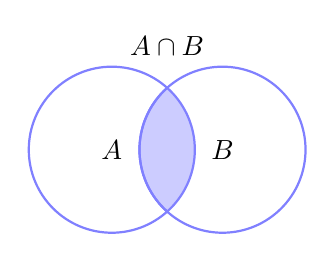
\begin{tikzpicture}
        \begin{scope}
            \clip \firstcircle;
            \fill[filled] \secondcircle;
        \end{scope}
        \draw[outline] \firstcircle node {$A$};
        \draw[outline] \secondcircle node {$B$};
        \node[anchor=south] at (current bounding box.north) {$A \cap B$};
    \end{tikzpicture}%
    %
    \hspace{2\baselineskip}%
    %
    % Set A or B
    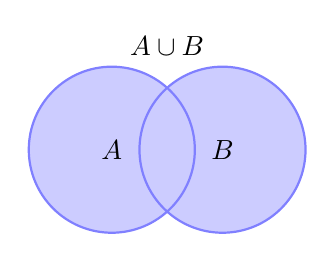
\begin{tikzpicture}
        \draw[filled] \firstcircle node {$A$}
                      \secondcircle node {$B$};
        \node[anchor=south] at (current bounding box.north) {$A \cup B$};
    \end{tikzpicture}

    %\hspace{2\baselineskip}%
    %
    % Set A but not B
    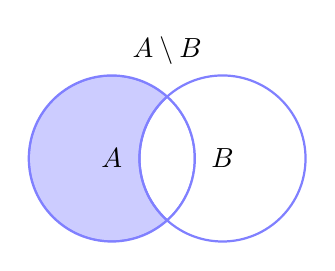
\begin{tikzpicture}
        \begin{scope}
            \clip \firstcircle;
            \draw[filled, even odd rule] \firstcircle node {$A$}
                                         \secondcircle;
        \end{scope}
        \draw[outline] \firstcircle
                       \secondcircle node {$B$};
        \node[anchor=south] at (current bounding box.north) {$A \setminus B$};
    \end{tikzpicture}%
    %
    \hspace{2\baselineskip}%
    %
    %Set A or B but not (A and B) also known a A xor B
    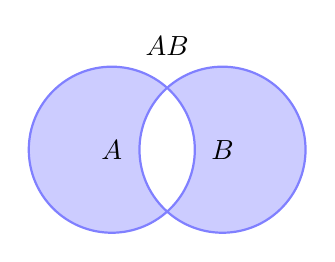
\begin{tikzpicture}
        \draw[filled, even odd rule] \firstcircle node {$A$}
                                     \secondcircle node{$B$};
        \node[anchor=south] at (current bounding box.north) {$A \symdiff B$};
    \end{tikzpicture}

    \caption{диаграммы Эйлера-Венна для двух пересекающихся множеств и результатов базовых операций с ними}
\end{figure}

\begin{figure}[ht!]
    \center
    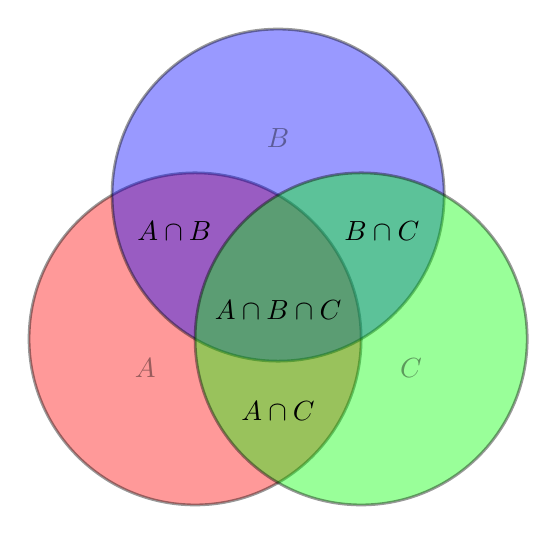
\begin{tikzpicture}
        \tikzset{venn circle/.style={draw,circle,minimum width=120pt,fill=#1,opacity=0.4,line width=1pt}}

        \node[venn circle = red] (A) at (0,0) {};% {$A$};
        \node[venn circle = blue] (B) at (60:60pt) {};% {$B$};
        \node[venn circle = green] (C) at (0:60pt) {};% {$C$};

        \node[text opacity=0.4] at (barycentric cs:A=7,B=-1,C=-1 ) {$A$};
        \node[text opacity=0.4] at (barycentric cs:A=-1,B=7,C=-1 ) {$B$};
        \node[text opacity=0.4] at (barycentric cs:A=-1,B=-1,C=7 ) {$C$};

        \node at (barycentric cs:A=1,B=1,C=-2/3 ) {$A \cap B$};
        \node at (barycentric cs:A=1,B=-2/3,C=1 ) {$A \cap C$};
        \node at (barycentric cs:A=-2/3,B=1,C=1 ) {$B \cap C$};
        \node at (barycentric cs:A=2,B=1,C=2 ){$A \cap B \cap C$};
    \end{tikzpicture}
    \caption{диаграмма Эйлера-Венна для трёх множеств}
\end{figure}

\FloatBarrier

\begin{remark}
    Интересно, что невозможно нарисовать диаграмму Эйлера-Венна, состоящую из окружностей (пусть и произвольного размера), для всех вариантов отношений между четырьмя и более множествами.
\end{remark}

Наконец, введём последнее обозначение, необходимое в этом разделе.
\begin{definition}
    \defemph{Множеством всех подмножеств} (или \defemph{булеаном}) некоторого множества $ A $ называется множество $ \mathcal{P}(A) = 2^A = \{ x \mid x \subseteq A \} $.
\end{definition}


\begin{Exercise}[counter=SecExercise]
    \noindent
    Задайте формально следующие множества:
    \begin{enumerate}[label=\arabic*)]
        \item Множество простых чисел.
        \item Множество всех отрезков на числовой прямой.
        \item Множество всех действительных корней всевозможных нетривиальных квадратных многочленов с целыми коэффициентами.
              Что изменится, если убрать условие на коэффициенты?
    \end{enumerate}
\end{Exercise}

\begin{Answer}
    \noindent
    \begin{enumerate}[label=\arabic*)]
    \item $ \mathbb{P} = \left \{ x \in \N \mid \neg \left( \exists a \exists b \, (x = a \cdot b) \wedge (a \neq 1) \wedge (a \neq x) \right) \wedge (x \neq 1) \right \} $.\\
        По умолчанию считаем, что $ a $ и $ b $ принадлежат тому же юнивёрсуму, что и $ x $.
    \item $ S = \left\{ x \in 2^{\R} \mid \exists a \exists b \, (a \in \R) \wedge (b \in \R) \wedge \left( \forall c \, (a \leqslant c \leqslant b) \leftrightarrow (c \in x) \right) \right\} $
    \item $ R = \left\{ x \in \R \mid \exists a \exists b \exists c \, (a \in \Z) \wedge (b \in \Z) \wedge (c \in \Z) \wedge (a^2 + b^2 + c^2 \neq 0) \wedge (a x^2 + b x + c = 0) \right\} $.\\
          Если коэффициенты сделать произвольными, то, очевидно, получится $ \R $, так как любое число $ a $ является корнем $ x - a = 0 $.
    \end{enumerate}
\end{Answer}


\begin{Exercise}[counter=SecExercise]
    \noindent
    Нарисуйте диаграмму Эйлера-Венна для трёх множеств из предыдущей задачи.
\end{Exercise}

\begin{Answer}
    \noindent
    Очевидно, $ S $ никак не пересекается с $ \mathbb{P} $ и $ R $ в силу разной природы объектов.
    Также понятно, что для любого простого числа $ p $ можно построить многочлен $ x - p $ с целыми коэффициентами, корнем которого $ p $ и будет являться;
    также, например, $ \sqrt{2} \in R $.
    Итого, $ \mathbb{P} \varsubsetneq R $.

    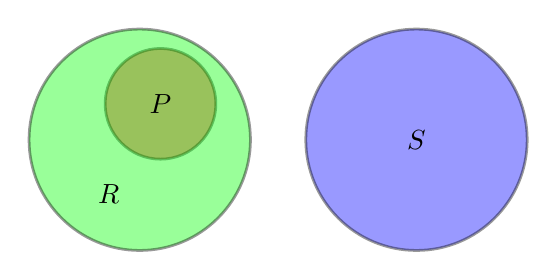
\begin{tikzpicture}
        \tikzset{venn circle/.style={draw,circle,minimum width=80pt,fill=#1,opacity=0.4,line width=1pt}}

        \node[venn circle = red, minimum width=40pt] (A) at (60:15pt) {};% {$A$};
        \node[venn circle = blue] (B) at (0:100pt) {};% {$B$};
        \node[venn circle = green] (C) at (0,0) {};% {$C$};

        \node at (barycentric cs:A=1,B=0,C=0 ) {$\mathbb{P}$};
        \node at (barycentric cs:A=0,B=1,C=0 ) {$S$};
        \node at (barycentric cs:A=-3,B=0,C=5 ) {$R$};
    \end{tikzpicture}
\end{Answer}


\begin{Exercise}[counter=SecExercise]
    \noindent
    Верно ли, что если $ B \subseteq A $, то $ A \setminus B = A \symdiff B $?
\end{Exercise}

\begin{Answer}
    \noindent
    Если $ B \subseteq A $, то
    \[
        \I_{A \symdiff B}(x) = \underbrace{(\I_A(x) \vee \I_B(x))}_{\I_A(x), \; \text{т.к.} \; \forall x \, \I_B(x) \rightarrow \I_A(x)} \wedge
        \underbrace{\neg (\I_A(x) \wedge \I_B(x))}_{\neg \I_B(x), \; \text{т.к.} \; \forall x \, \I_B(x) \rightarrow \I_A(x)} =
        \I_A(x) \wedge \neg \I_B(x) = \I_{A \setminus B}(x)
    \]
    Аналогичное доказательство в теоретико-множественных обозначениях:
    \[
        A \symdiff B = \underbrace{(A \cup B)}_{A} \setminus \underbrace{(A \cap B)}_{B} = A \setminus B
    \]
    Наконец, проведём также лобовое доказательство через проверку тавтологичности следующей формулы:
    \[
        (b \rightarrow a) \rightarrow \left( (a \wedge \neg b) \leftrightarrow (a \oplus b) \right)
    \]
    Здесь введены обозначения $ a = \I_A(x) $, $ b = \I_B(x) $.
    Используя закон де Моргана, а также тождества $ x \to y = \neg x \vee y $ и $ x \oplus y = \neg (x \leftrightarrow y) $, перепишем формулу в виде
    \[
        (b \rightarrow a) \rightarrow \left( \neg (a \rightarrow b) \leftrightarrow \neg (a \leftrightarrow b) \right)
    \]
    Операция <<$ \leftrightarrow $>> позволяет убрать отрицания с обоих аргументов:
    \[
        (b \rightarrow a) \rightarrow \left( (a \rightarrow b) \leftrightarrow (a \leftrightarrow b) \right)
    \]
    Воспользуенмся дистрибутивностью импликации относительно эквивалентности (см. конец решения задачи \ref{ex:boolean:disjunction_distributivity_over_equivalence}):
    \[
        \left[ (b \rightarrow a) \rightarrow (a \rightarrow b) \right] \leftrightarrow \left[ (b \rightarrow a) \rightarrow (a \leftrightarrow b) \right]
    \]
    Перепишем эквивалентность в последней скобке через конъюнкцию импликаций
    и воспользуемся дистрибутивностью импликации относительно конъюнкции:
    \[
        \left[ (b \rightarrow a) \rightarrow (a \rightarrow b) \right] \leftrightarrow \left[ (b \rightarrow a) \rightarrow \left( (a \rightarrow b) \wedge (b \rightarrow a) \right) \right]
    \]
    \[
        \left[ (b \rightarrow a) \rightarrow (a \rightarrow b) \right] \leftrightarrow
        \left[ \left( (b \rightarrow a) \rightarrow (a \rightarrow b) \right) \wedge \left( (b \rightarrow a) \rightarrow (b \rightarrow a) \right) \right]
    \]
    Второй операнд конъюнкции тавтологичен, и формула, наконец, упрощается:
    \[
        \left[ (b \rightarrow a) \rightarrow (a \rightarrow b) \right] \leftrightarrow
        \left[ (b \rightarrow a) \rightarrow (a \rightarrow b) \right]
    \]
    Здесь тавтологичность уже очевидна в силу равенства формул для левой и правой частей.
\end{Answer}

Третий способ доказательства в предыдущей задаче получился самым громоздким, но самым формальным,
а потому подвластным компьютеру (см. автоматические доказательства теорем).
Более того, в нём еще раз было продемонстрировано красивое свойство логики~---
возможность формально описывать саму себя на своём языке.

\begin{Exercise}[counter=SecExercise]
    \noindent
    Используя только операции $ \symdiff $ и $ \cap $, выразите $ A \cup B \cup C $
\end{Exercise}

\begin{Answer}
    \noindent
    Докажем, что
    \[
        A \cup B \cup C = U \symdiff A \symdiff B \symdiff C \symdiff A \cap B \symdiff A \cap C \symdiff B \cap C \symdiff A \cap B \cap C
    \]
    Действительно, если это переписать в терминах индикаторных функций, то получим
    \[
        %1 \oplus \I_A(x) \oplus \I_B(x) \oplus \I_C(x) \oplus \I_A(x) \wedge \I_B(x) \oplus \I_A(x) \wedge \I_C(x) \oplus \I_B(x) \wedge \I_C(x) \oplus \I_A(x) \wedge \I_B(x) \wedge \I_C(x)
        1 \oplus a \oplus b \oplus c \oplus a \wedge b \oplus a \wedge c \oplus b \wedge c \oplus a \wedge b \wedge c
    \]
    где $ a = \I_A(x) $, $ b = \I_B(x) $, $ c = \I(x) $.

    Видно, что если $ a = b = c = 0 $, то выражение ложно.
    Также заметим, что если $ a = 1 $, а $ b = c = 0 $, то выражение истинно.
    Далее можно заметить, что до тех пор, пока есть хотя бы одна истинная переменная, формула не меняет своего значения при изменении любой другой переменной:
    свои значения всегда будет менять чётное число слагаемых.
    Но тогда из всего вышесказанного следует, что формула задаёт функцию $ a \vee b \vee c $.
    Возвращаясь к множествам, получаем, что исходное тождество доказано.

    Кратко упомянем и иное доказательство: достаточно проверить равенство только в случаях $ (a,b,c) = (0,0,0) $, $ (1,0,0) $, $ (1,1,0) $ и $ (1,1,1) $, а потом воспользоваться симметричностью формулы.
\end{Answer}


\iffalse
\subsection{Мощность множества}
\label{subsec:sets:cardinality}

Помимо состава множеств и взаимоотношений между ними нас часто будет интересовать то, насколько некоторое множество <<велико>>.
Легко определить <<размер>> множества в случае, когда оно конечно: это просто число элементов.
Но что делать, если множество содержит бесконечно много элементов?
Хочется сказать, что если два множества бесконечны, то они <<равновелики>>.
Однако это противоречит интуитивным представлениям о том, что, например, $ 2^A $ содержит элементов больше, чем $ A $.

Оказывается, эти интуитивные представления можно формализовать, если по-другому взглянуть на размер конечных множеств.
Если множества $ A $ и $ B $ конечны, то можно сказать, что они равновелики, если в них одинаковое число элементов.
По сути, это эквивалентно тому, что можно задать взаимнооднозначное правило соответствия между каждым элементом $ A $ и $ B $.
%достаточно пронумеровать элементы любым способом, и в соответствие друг другу ставить элементы с одинаковым номером;
%обратное следствие тоже очевидно: если мы пронумеруем элементы одного множества, то, благодаря правилу, будут пронумерованы элементы и другого множества,
%причём не будет ни повторений, ни пропущенных элементов.

\begin{statement}
    Если $ A $ и $ B $~--- конечные множества, то они содержат одинаковое число элементов тогда и только тогда,
    когда существует взаимнооднозначное соответствие (\defemph{биекция}) между элементами множеств.
\end{statement}

Формальное доказательство утверждения становится очевидным, если любым способом пронумеровать элементы множеств.

Данное утверждение позволяет по-иному формально определить размер, или \defemph{мощность} множества, и обобщить это определение на все множества вообще.
\begin{definition}
    Множества $ A $ и $ B $ называются \defemph{равномощными} в том и только том случае,
    если существует взаимнооднозначное соответствие между элементами множеств.
\end{definition}
Стоит обратить внимание, что формальное определение взаимнооднозначного соответствия будет дано гораздо позже.
Также понятно, что это соответствие не обязано быть единственным.

\begin{definition}
    Множество $ A $ называется \defemph{счётным} $ \defarr $ $ A $ равномощно $ \N_0 $.
\end{definition}

\begin{example}
    \begin{enumerate}
        \item[]
        \item
            Множества $ \{1, 2\} $ и $ \{a, x\} $ равномощны, причём можно построить два взаимнооднознычных соответствия между ними:
            \[
                1 \sim a, \; 2 \sim x \qquad \text{или} \qquad 1 \sim x, \; 2 \sim a
            \]
        \item
            Множества $ \N_0 $ и $ E = \{ x \in \N_0 \mid \exists k \, (x = 2k) \} $ равномощны, соответствие задаётся, например, правилом $ E \ni x = 2 \cdot k $, где $ k $~--- любой элемент $ \N_0 $.
        \item
            Множества $ \Q $ и $ \N_0 $ равномощны.
            Идея доказательства: $ \Q $ можно задать бесконечной таблицей, номер строки и столбца в которой~--- числитель и знаменатель.
            А все ячейки таблицы можно пронумеровать, идя <<змейкой>> (при этом сократимые дроби не нумеруются).
    \end{enumerate}
\end{example}

Может создасться впечатление, что все бесконечные множества счётны.
Однако это неверно.

\begin{theorem}[Кантора]
    Для любого $ A $ множества $ A $ и $ 2^A $ неравномощны.
\end{theorem}

\begin{statement}
    Множество $ \R $ несчётно.
\end{statement}

Доказательство данного утверждения обычно приводят в курсе математического анализа.

\begin{Exercise}[counter=SecExercise]
    \noindent
    Счётно ли множество всех корректных программ, написанных на языке C++?
\end{Exercise}

\begin{Answer}
    \noindent
    Да, оно счётно.
    Для доказательства этого заметим, что можно построить следующую таблицу:
    номер строки равен длине программы в символах, а номер столбца~--- лексикографическому порядковому номеру программы среди всех программ заданной длины.
    Обходя таблицу <<змейкой>>, получаем взаимнооднозначную нумерацию всех программ.
\end{Answer}
\fi
